\subsection{Overview of the implementation architecture[Md Jahidul Haque]}\label{sec:arch-aws}
In order to implement the CI/CD pipeline for our spring boot application, we needed a technology to choose for the repository management. In this case, we used the GitHub Actions for the repository management. Unlike codeCommit from AWS, Github Action is free to use and this way we cover up our cost of implementation. We have used GitHub's DSl to setup the configuration scripts in {{.yml}} files. 

The CI is managed via the {{.yml}} file of our code base. To simplify our tasks for automating the infrastructure objects we used node package manager(npm) to setup the necessary commands for the pipeline.

The CD pipeline of the SDLC means the automation of the release processes which are related with automatic deployment environment, network configuration and infrastructure object creation. For automating deployment environment, Github actions can be used to describe the environment definitions to create resources that are needed for the application. Then other batch jobs execute deployment environment and test the application via acceptance testing. 

After successful deployment, the infrastructure objects creation are defined via CloudFomation's  cloud development kit(CDK). In this CDK, we can define Java classes for describing the infrastructure objects and then that objects can be compiled via AWS's CLI. All the infrastucture automation commands is included in the Github actions so that infrastructure objects can automatically be created via {{.yml}} scripts.











In our implementation, we used several technology to automate the software release. Beside using Github Actions, we also used docker file to create deployment environment and AWS CloudFormation for continuous delivery. The figure ~\ref{fig:ci-cd} describes all the github steps that we created in the pipeline implementation for AWS based spring boot application.

\begin{figure}[h]
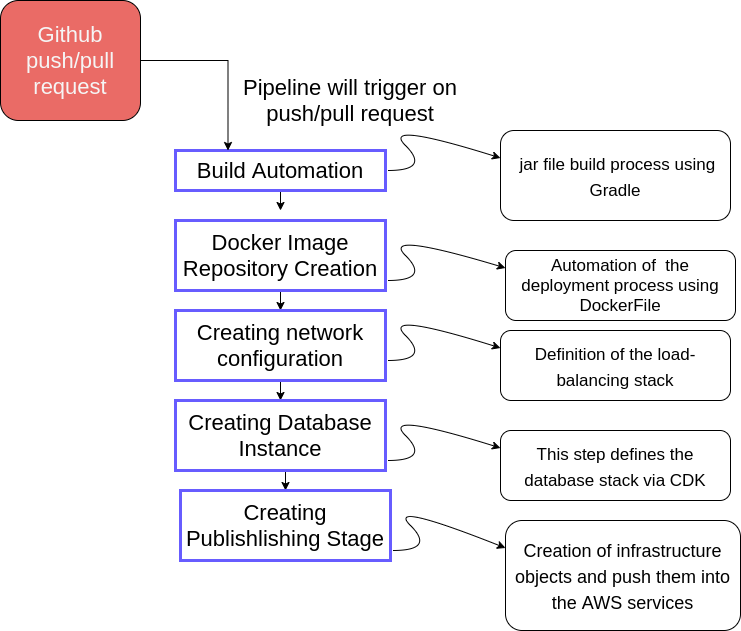
\includegraphics[scale=0.60]{images/jahidul/arch_ci_cd.png}
\centering
\caption{The {{CI\CD}} pipeline Architecture for AWS Cloud-native Application}
\label{fig:ci-cd}
\end{figure}

In the Figure.~\ref{fig:ci-cd} the triggering mechanism is indicated which briefs the pipeline orchestration on push or pull request of the project's repository. In order to maintain branch operation we defined the designated branch to pick in the job definition so that github workflow can checkout the defined branch in the {{.yml}} file. When the push is triggred in the designated branch in the {{.yml}} file, the build process starts as shown in the figure \ref{fig:ci-cd} and then other task are initiated accordingly. In this project, we implement five key tasks for the spring-boot application. For deployment automation at first we implemented a CI/CD pipeline architecture using Github Actions. Then we secured our DNS of the service via implementing the SSL certificated via letsencrypt inside the AWS ECS container. After securing our DNS we developed a new service of the application to test the whole pipeline. During the development of the service we have created integration tests, unit tests using JUNIT5. In this implementation, we also enable PostgreSQL configurations inside the AWS's RDS container for maintaining the persistence data. After developing the new modification of the software, we implemented the whole infrastructure automation using the CDK of AWS's CloudFormation.